%\addcontentsline{toc}{chapter}{Simulator Jitter}\label{ch:SimJitter}
\chapter{Simulator Jitter}
\label{ch:SimJitter}

\section{Context}
During the testing of the NAMURU receiver, issues with the performance were identified. In particular, the receiver was failing to sustain phase-lock, resulting in an inability to track the signal. By conducting a thorough investigation using the KeaDebug feature, the source of the excessive phase error was uncovered, and the problem was rectified. 

\section{Investigation}

\begin{figure}[!htb] 
    \centering
    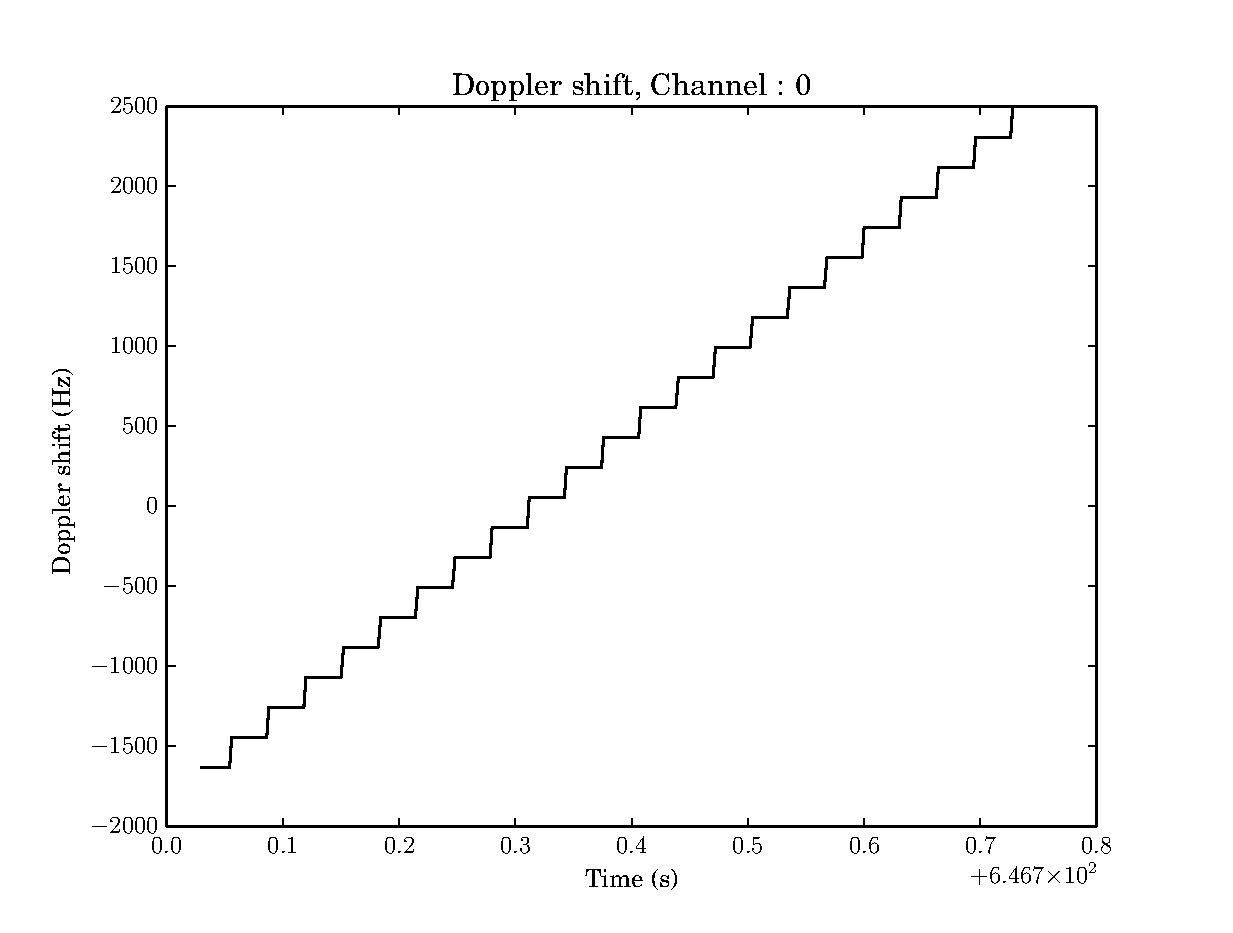
\includegraphics[width=1\textwidth]{SimulatorJitter/Stepping.eps} 
    \caption{The stepping pattern observed in the frequency output of the receiver.}
    \label{fig:Stepping}
\end{figure}

Upon examining the signal generated by the simulator, a discrete, quantised pattern became evident in the frequency output. This pattern, an example of which can be seen in \ref{fig:Stepping} resulted in excessive acceleration and jerk on a periodic basis, as opposed to constant acceleration, with zero jerk. Given the type 3 tracking loops in the receiver are sensitive to jerk, the root cause of the excessive phase error had been identified. By referring to the associated manuals for the GNSS simulators owned by the school, It became apparent that the GNSS simulate had a 10Hz update rate. By adjusting the update rate, the issue was rectified, however the actual impact of the step input on the receiver provided a unique insight to its operation.

In figures \ref{DopplerShiftSubsection0} and \ref{fig:PhaseAngleSubsection}, the impact of the stepping on the frequency and phase respectively can be identified. In both cases, the underdamped nature of the control system is evident. 

\begin{figure}[!htb] 
    \centering
    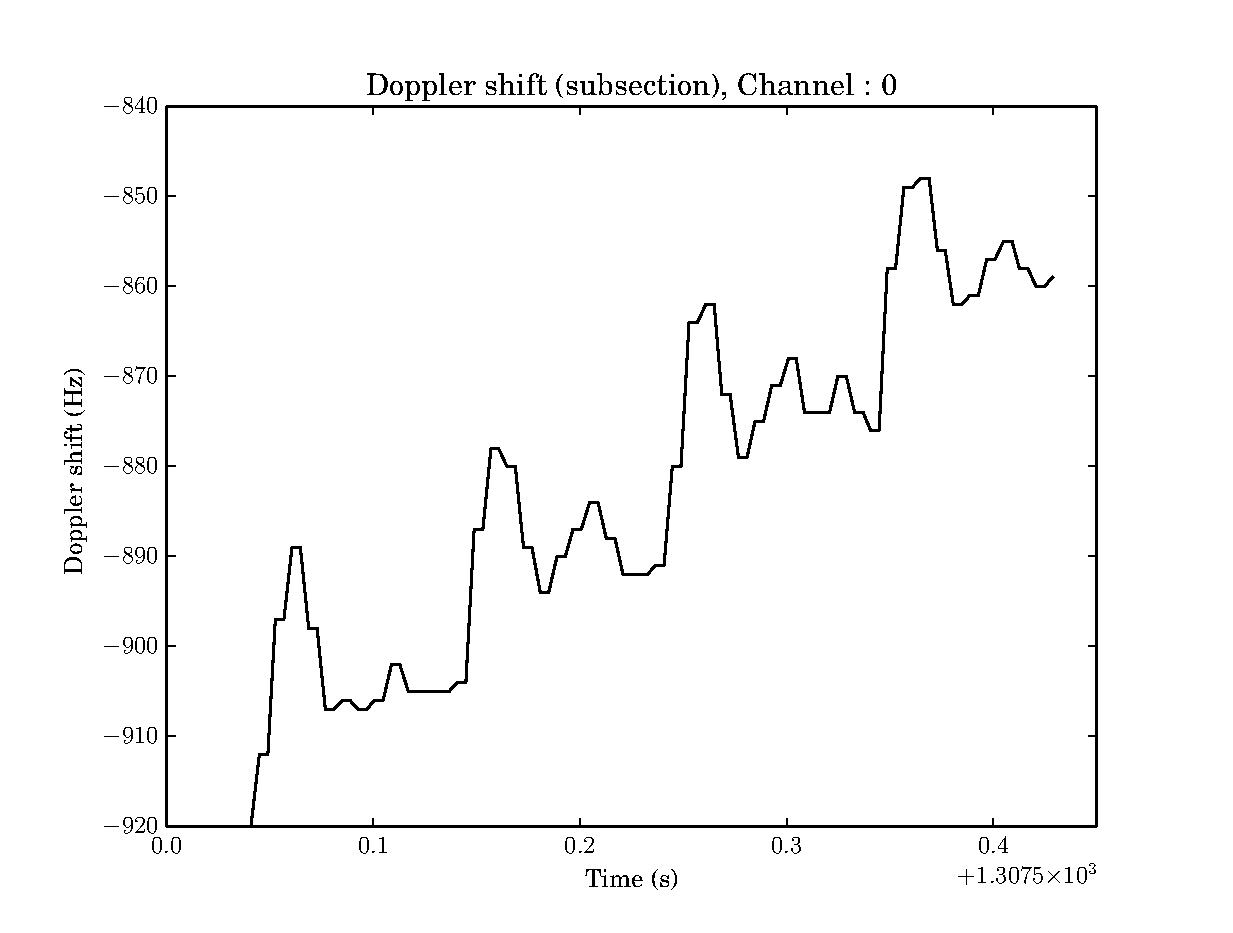
\includegraphics[width=1\textwidth]{SimulatorJitter/DopplerShiftSubsection0.eps} 
    \caption{The output from the receiver tracking loops. Notice the transient response to the step input in frequency.}
    \label{fig:DopplerShiftSubsection0}
\end{figure}

\begin{figure}[!htb] 
    \centering
    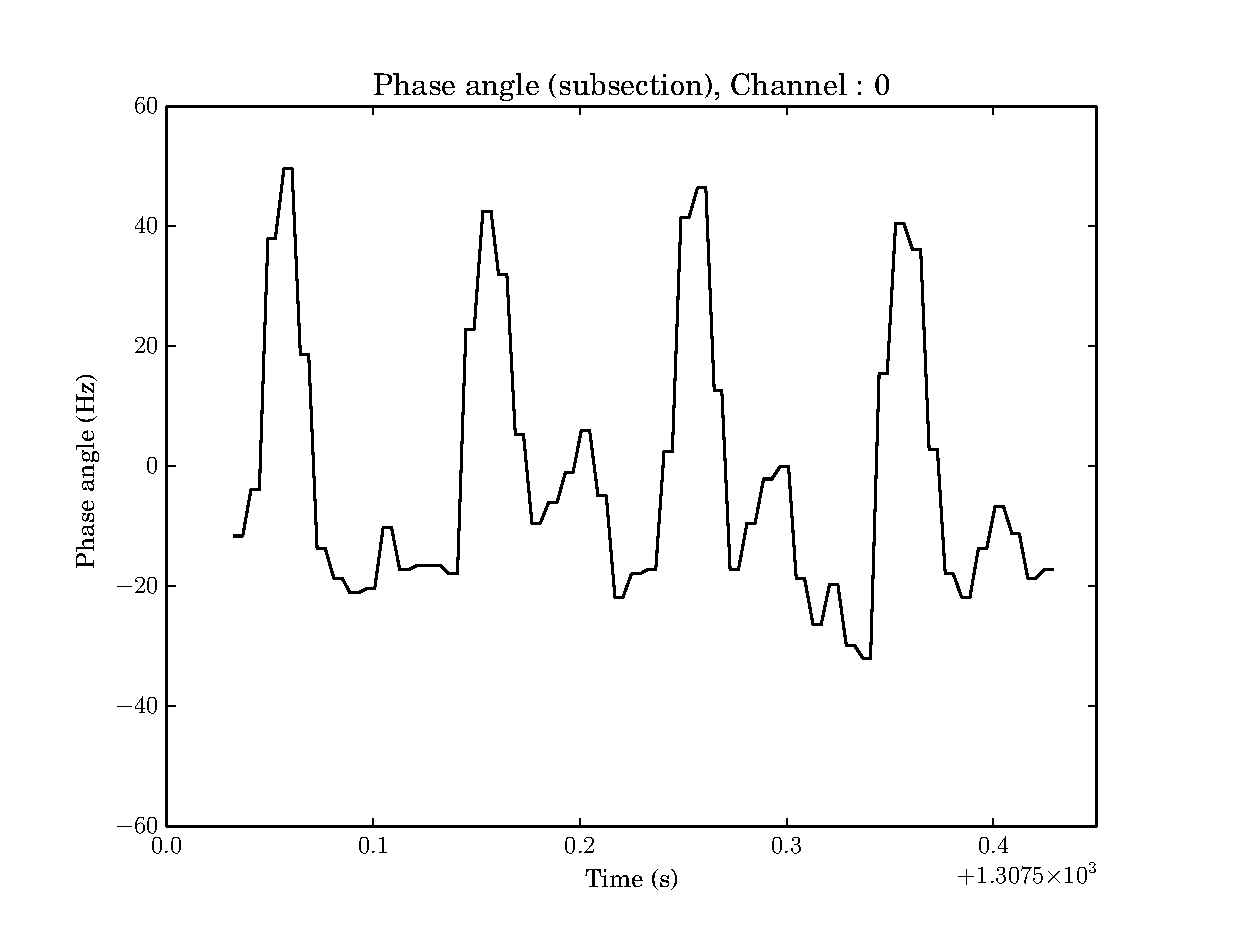
\includegraphics[width=1\textwidth]{SimulatorJitter/PhaseAngleSubsection0.eps} 
    \caption{In the phase output, the transient response, which resulted in the bimodal distribution of the phase angle is evident.}
    \label{fig:PhaseAngleSubsection0}
\end{figure}

\begin{figure}[!htb] 
    \centering
    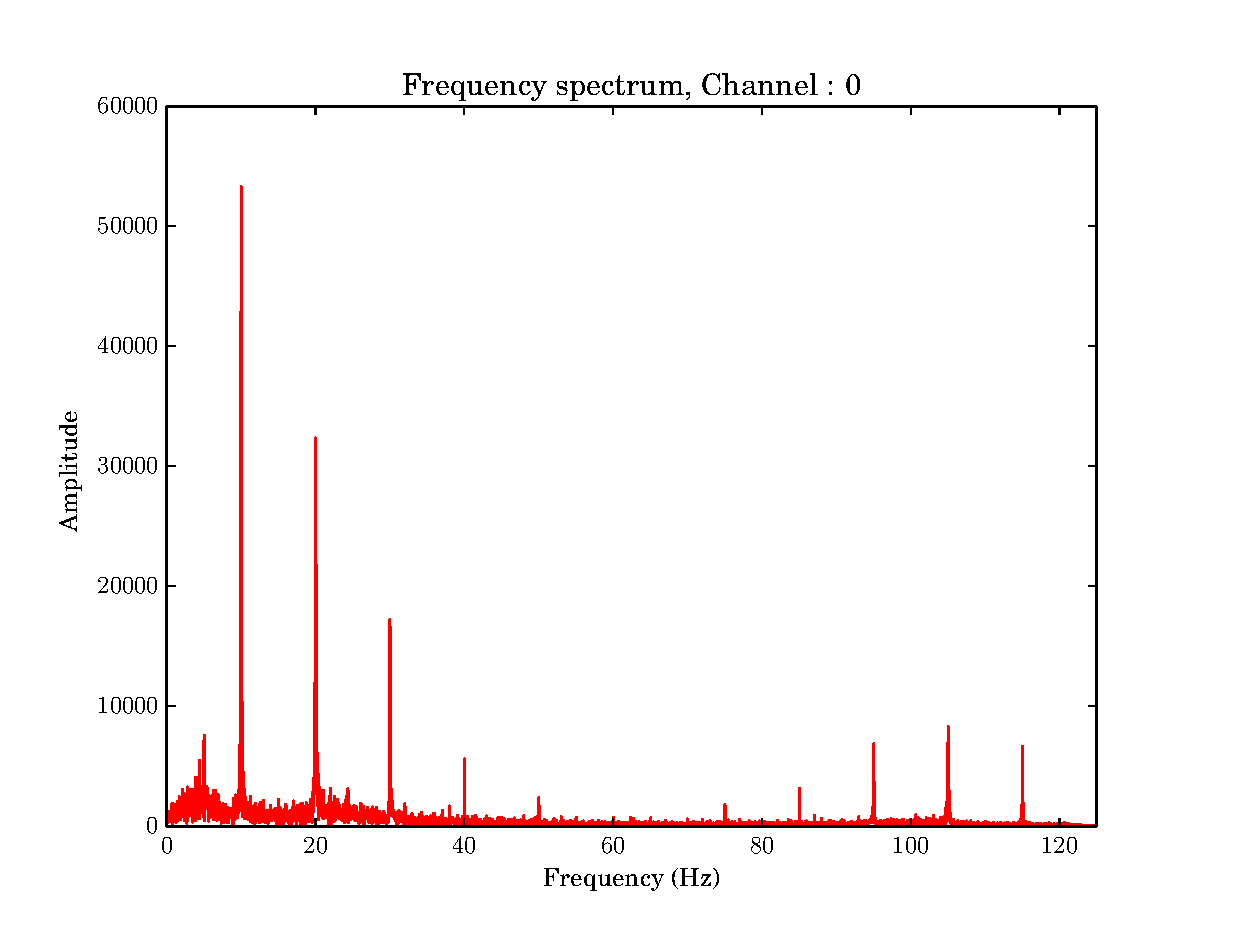
\includegraphics[width=1\textwidth]{SimulatorJitter/FFT0.eps} 
    \caption{The frequency spectrum of the phase errors, note the significant frequency component at 10Hz, and it's harmonics. This component is due to the 10Hz update rate of the simulator.}
    \label{fig:FFT0}
\end{figure}


\begin{figure}[!htb] 
    \centering
    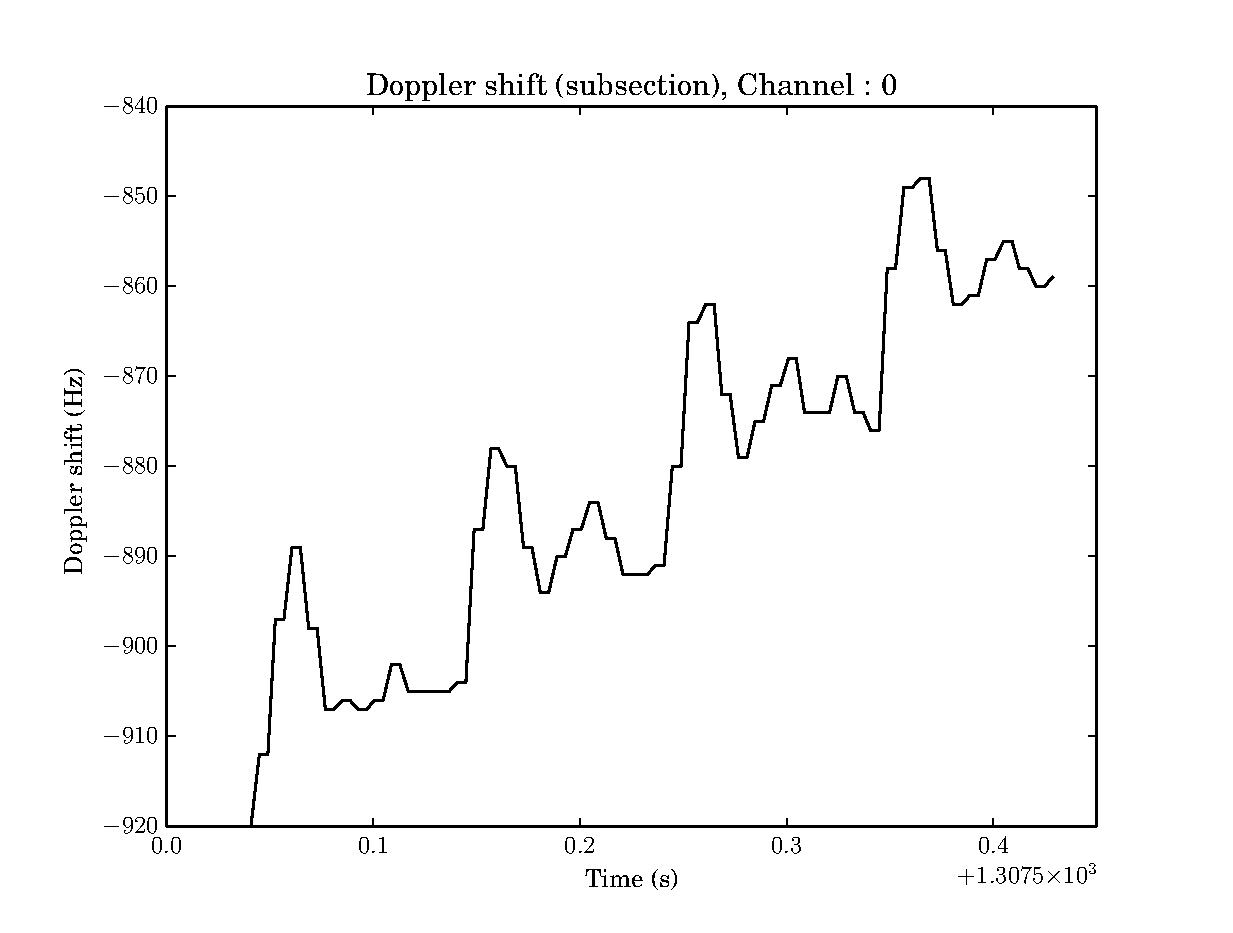
\includegraphics[width=1\textwidth]{SimulatorJitter/DopplerShift0.eps} 
    \caption{}
    \label{fig:DopplerShift0}
\end{figure}


\begin{figure}[!htb] 
    \centering
    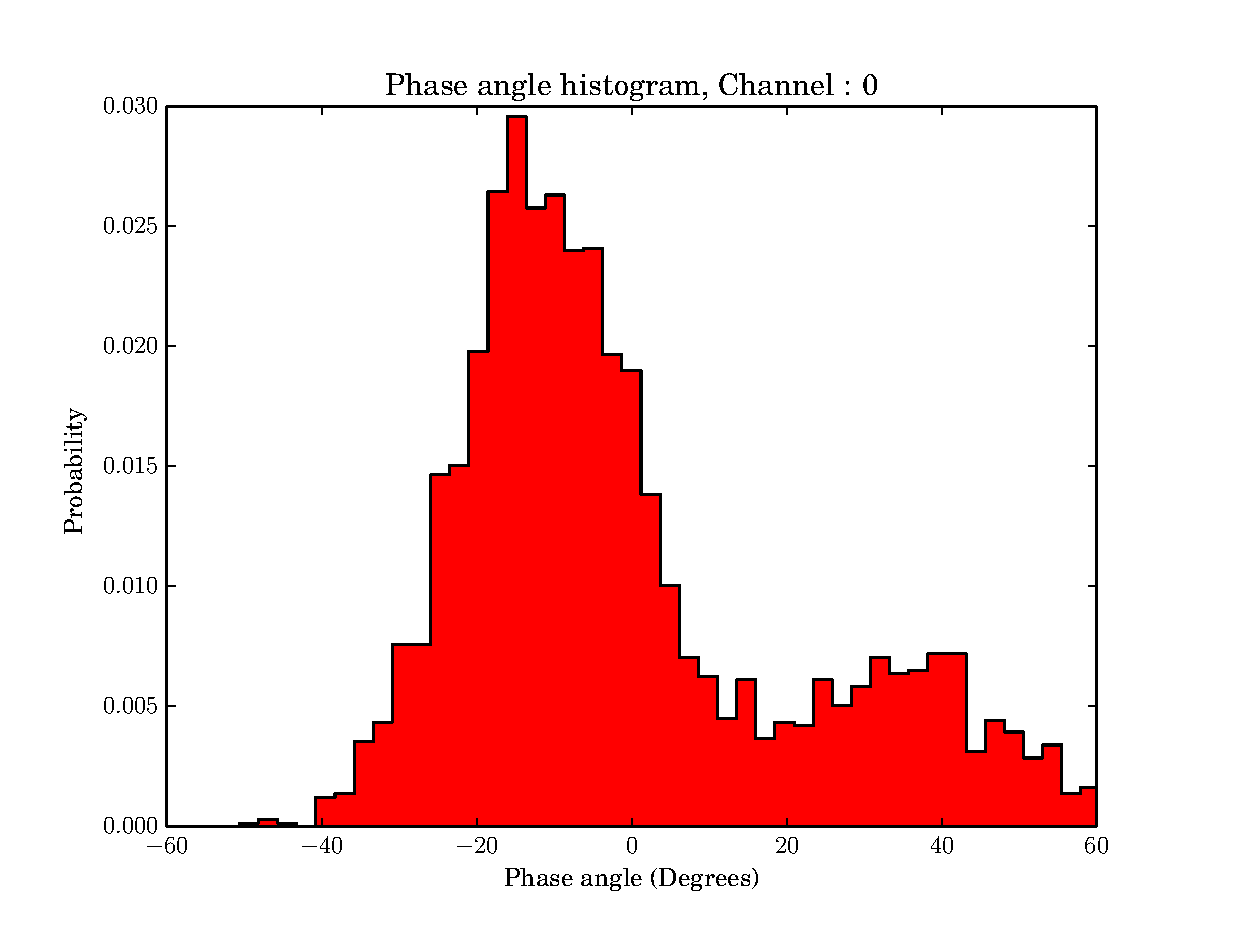
\includegraphics[width=1\textwidth]{SimulatorJitter/PhaseAngleHistogram0.eps} 
    \caption{A histogram of the phase errors. Notice the bimodal nature of the histogram, as opposed to the normal distribution that can be observed in figure \ref{fig:PhaseAngleHistogramStationary}.}
    \label{fig:PhaseAngleHistogram0}
\end{figure}

\begin{figure}[!htb] 
    \centering
    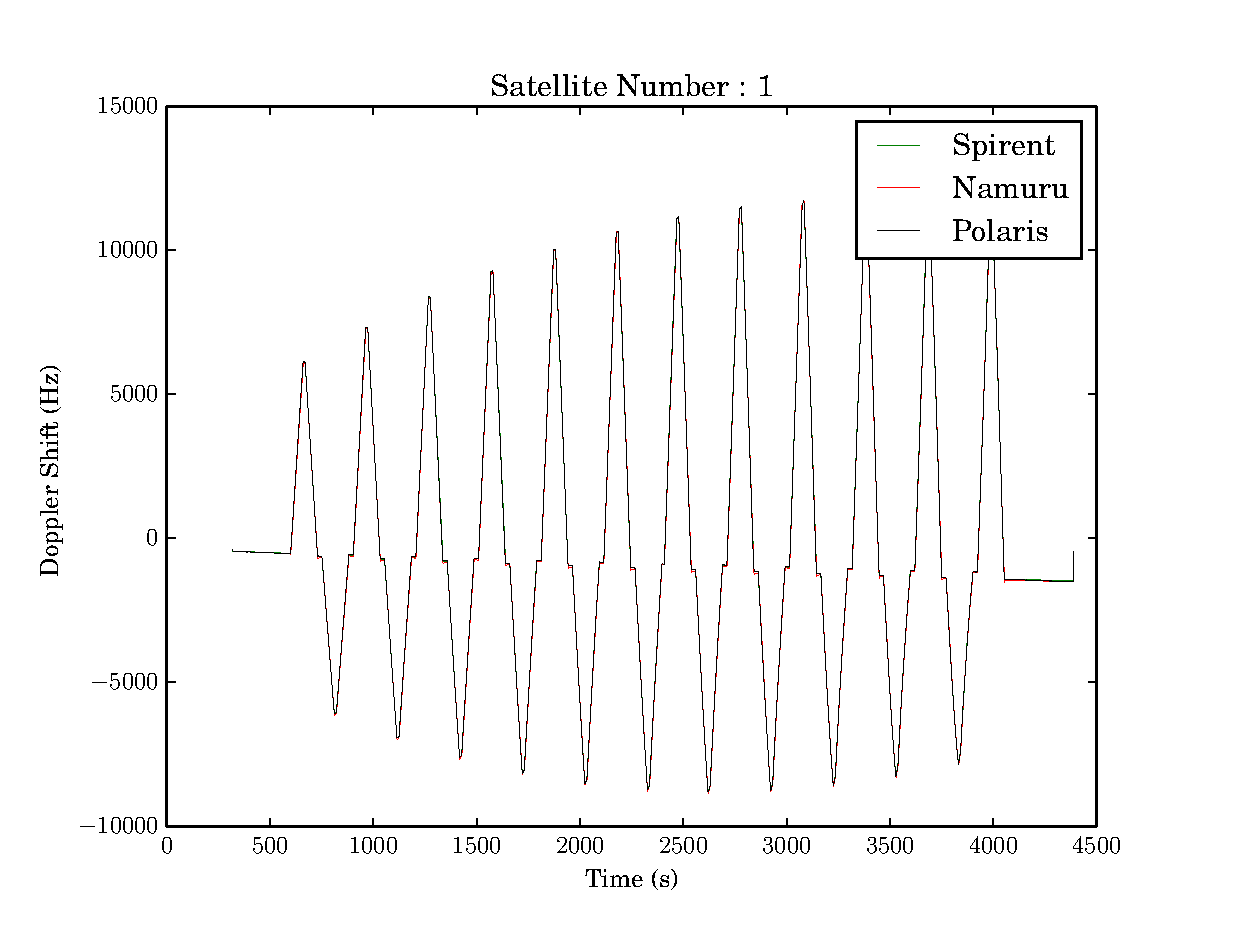
\includegraphics[width=1\textwidth]{SimulatorJitter/1Polaris.eps} 
    \caption{A comparison between the PLL outputs for Spirent, Namuru and Polaris. The Spirent output is the ground truth used in the simulation. The peak \ac{LOS} velocity achieved is approximately 2300m/s.}
    \label{fig:1Polaris}
\end{figure}



